%!TEX root = ../thesis-main.tex

\chapter{Analisi}

\section{Requisiti}

Il progetto si pone due principali obiettivi:
\begin{itemize}
	\item La generazione automatica di pacchetti di installazione multi-piattaforma \\ con \ac{jre} integrato.
	\item La pubblicazione automatica dei rilasci del software all'interno di repository pubblici selezionati.
\end{itemize}
Un pacchetto software è un insieme di risorse necessarie per eseguire un'applicazione o un servizio su un sistema. Sono usualmente distribuiti all'interno di archivi compressi contenenti meta-dati che ne descrivono la forma e l'utilizzo. La pubblicazione è l'atto di inserire il software in archivi (repository) online con l'intento di consentire l'installazione agli utenti finali. Entrambi i processi devono essere automatizzati ed integrati all'interno di una pipeline di integrazione e rilascio continua.

\paragraph{Requisiti funzionali}

Le funzionalità richieste si possono classificare in due gruppi distinti: il primo contiene tutto ciò che concerne l'esperienza dell'utente finale, mentre il secondo descrive le funzionalità dal punto di vista degli sviluppatori e contributori di Alchemist. Di seguito il primo gruppo.
\begin{itemize}
	\item \textbf{Pacchettizzazione}: il simulatore deve essere distribuito in pacchetti auto-contenuti, ossia comprendenti di tutto il necessario per l'utilizzo di esso.
	\item \textbf{Multi-piattaforma}: Alchemist deve essere installabile sui maggiori sistemi operativi in circolazione come Windows, MacOS e le principali distribuzioni Linux.
	\item \textbf{Plug and play}: l'installazione non deve richiedere configurazioni complesse, l'applicativo deve essere pronto all'uso non appena installato.
\end{itemize}

I requisiti del gruppo successivo sono accumunabili per il loro scopo, vale a dire l'automazione.

\begin{itemize}
	\item \textbf{Automazione dei pacchetti}: la generazione dei pacchetti di installazione deve essere automatica e configurabile.
	\item \textbf{Automazione della distribuzione}: il rilascio di una nuova versione comprende la distribuzione di essa nei repository selezionati e deve essere svolta in modo automatico.
	\item \textbf{Verifica funzionamento}: entrambi i processi descritti precedentemente devono essere corredati da verifiche del loro funzionamento e devono bloccare la procedura di rilascio nell'eventualità siano presenti errori.
\end{itemize}

\paragraph{Requisiti non funzionali}

\begin{itemize}
	\item Trattandosi Alchemist di un software in continuo sviluppo, è auspicabile l'utilizzo degli strumenti già impiegati nel progetto. \\ L'integrazione di nuovi applicativi deve essere eseguita solo se strettamente necessaria.
	\item La pipeline \ac{cicd} ottenuta deve garantire prestazioni in linea con la versione precedente l'intervento di questo progetto.
\end{itemize}

\section{Pacchettizzazione}\label{sec:packaging}

Come si evince dall'analisi svolta, la pacchettizzazione è un requisito fondamentale dell'elaborato. Sino ad ora l'applicativo Alchemist era distribuito in file JAR, ossia archivi java compressi contenenti tutte le dipendenze ed i relativi \textit{classfiles} necessari all'esecuzione. Quest'approccio molto diffuso porta con sè diverse limitazioni tra cui:
\begin{itemize}
	\item la necessità dell'utente scaricante di avere un \ac{jre} installato nel proprio dispositivo;
	\item il potenziale bisogno di utilizzare un ambiente \ac{jre} specifico e quindi per l'utente di non possedere una versione dell'ambiente compatibile;
	\item la difficoltà di utilizzo per utenti non esperti, i quali sono abituati ad eseguire programmi utilizzando file eseguibili nativi della propria piattaforma.
\end{itemize}
Alcune di queste restrizioni risultano mitigate, tuttavia non in tutte le piattaforme come Windows, il quale per esempio non fornisce un ambiente java pre-installato. Esistono diversi strumenti di terze parti e non che cercano di far fronte a questo problema, è importante dunque valutare e scegliere lo strumento più opportuno.

\subsection{Soluzioni}

Nell'ottica di semplificare la configurazione di questo processo lo strumento selezionato deve supportare le tre principali piattaforme descritte nei requisiti precedentemente. Tra gli strumenti analizzati due molto differenti si sono distinti, vale a dire: \textit{jpackage}, comando disponibile nel \ac{jdk} dalla versione 14, adibito alla produzione di pacchetti auto-contenuti con \ac{jre} integrata e \textit{GraalVM}, un \ac{jdk} sviluppato da Oracle che fornisce un compilatore \ac{jit} e \ac{aot} per java. 

Il termine \ac{jit} descrive il comportamento normale di ogni \ac{jvm}: il \textit{java compiler} traduce il programma ad alto livello in \textit{bytecode} ed in seguito la \ac{jvm} trasforma il bytecode in linguaggio macchina per l'architettura specifica dinamicamente. In contrasto la tecnica \ac{aot} ricorda i linguaggi di programmazione compilati, ovvero la compilazione è statica ed avviene prima dell'esecuzione del programma. Il compilatore \ac{aot} chiamato ``Native Image", consente di compilare un programma java (ed altri linguaggi di programmazione) ottenendo in output un eseguibile nativo per ogni piattaforma. Quest'ultimo inoltre porta con sè diversi vantaggi come: un minor costo in risorse CPU e memoria, tempi di avvio minori e dimensioni ridotte rispetto un normale programma java distribuito con un \ac{jre}. La compilazione \ac{aot} però ha dei requisiti, uno di questi fondamentale è la \textit{closed world assumption}: ossia ogni parte di codice raggiungibile in esecuzione lo deve essere anche in fase di build. Ciò accade perché native image svolge un analisi statica del codice, alcune funzionalità come la reflection oppure il caricamento dinamico non sono supportate e richiedono una soluzione alternativa.

In contrasto jpackage fornisce uno strumento interessante, il quale non richiede modifiche all'applicativo ed è pre-installato in tutti i \ac{jdk} dalla versione 14 e successive. Supporta nativamente l'annessione di un \ac{jre} utilizzando \textit{jlink}, produce diverse tipologie di pacchetti per ogni piattaforma ed è completamente controllabile da interfaccia \ac{cli}. Le tipologie di pacchetti generabili sono elencate di seguito:
\begin{itemize}
	\item \textit{exe} e \textit{msi} per Windows;
	\item \textit{rpm} e \textit{deb} per Linux;
	\item \textit{pkg} e \textit{dmg} per MacOs.
\end{itemize}
Tuttavia anch'esso presenta dei limiti come: la necessità di essere eseguito sullo stesso sistema operativo dove i pacchetti prodotti sono destinati (lo stesso vale per GraalVM, la \textit{cross compilation} non è supportata) e la produzione di un solo pacchetto per singola esecuzione.

\paragraph{Valutazione finale} Ambedue le soluzioni, seppure differenti concorrono all'obiettivo primario, la distribuzione del software multi-piattaforma. GraalVM fornisce diversi vantaggi prestazionali, ma i requisiti da esso richiesti non sono compatibili con l'architettura del simulatore. D'altro canto jpackage fornisce tutto il necessario per costruire i pacchetti con embed di un \ac{jre} senza la necessità di stravolgere l'architettura del software, ed i limiti delineati sono superabili adoperando script o configurazioni specifiche.

\section{Strumenti}

\subsection{Gradle}

Mentre in passato la produzione di artefatti (documentazione, pacchetti, eseguibili) era delegata a script costruiti dallo sviluppatore, in un progetto di grandi dimensioni è oggigiorno essenziale avvalersi di uno strumento di \textit{build automation}. Come l'output di un programma deterministico non cambia per uno stesso input, la produzione di artefatti deve essere consistente e riproducibile riducendo al minimo l'intervento umano. 

Gradle\footnote{https://gradle.org/} è uno dei tanti strumenti disponibili, supporta diversi linguaggi di programmazione anche se risulta popolare nell'ambiente JVM come alternativa a Maven. I \textit{task} sono l'unità minima di esecuzione e rappresentano un azione: come generare un JAR, eseguire dei test o produrre la documentazione. Mediante direttive come \textit{dependsOn} è possibile creare dipendenze tra processi: Gradle orchestra l'esecuzione dei task costruendo un grafo aciclico diretto (DAG) delle dipendenze. L'esecuzione di Gradle avviene in tre fasi distinte elencate di seguito.
\begin{enumerate}
	\item \textbf{Fase di inizializzazione}: in primo luogo Gradle crea un'istanza di Settings che organizza l'architettura del progetto. Attraverso un file, di nome ``settings.gradle", lo sviluppatore stabilisce il progetto radice e tutti gli eventuali progetti figli. 
	\item \textbf{Fase di configurazione}: successivamente tutti i file di configurazione ``build\-.\-gradle" (del progetto radice e tutti i sotto-progetti) vengono analizzati per costruire il grafo dei task.
	\item \textbf{Fase di esecuzione}: infine, Gradle esegue i task richiesti considerando le dipendenze descritte nel grafo generato nella fase precedente.
\end{enumerate}

\imagesource{figures/gradle-build-lifecycle-example.png}{https://docs.gradle.org/current/userguide/build_lifecycle.html}{Esempio di inizializzazione, configurazione ed esecuzione di una build Gradle}{1}{gradle-build-lifecycle}

Un componente chiave sono i plugin, i quali consentono di estendere le funzionalità di Gradle: aggiungere nuovi task, estendere il modello con nuovi elementi ed applicare configurazioni specifiche all'intero progetto. La presenza di diversi plugin base e creati dalla comunità rende Gradle uno strumento versatile.

\paragraph{Analisi rispetto ai requisiti}
In considerazione dei requisiti di automazione, Gradle fornisce le funzionalità necessarie a soddisfare i requisiti di pacchettizzazione, distribuzione e verifica del funzionamento. Utilizzando Gradle si integrano questi processi all'interno del build system garantendo un corretto ordine di esecuzione con l'effetto di minimizzare l'incidenza di errori e assicurando la produzione di pacchetti conformi su qualsiasi sistema operativo questo venga eseguito.
L'approccio orientato ai task inoltre permette di suddividere un macro-processo in più unità di esecuzione riutilizzabili da altri processi, garantendo tutti i vantaggi che la filosofia \ac{dry} fornisce.

\subsection{GitHub Actions}

Tramite Gradle lo sviluppatore è in grado di eseguire procedure articolate come compilazione, test e dispiegamento utilizzando un semplice comando da \ac{cli}. L'invocazione di queste procedure richiede però l'intervento umano, è quindi necessario uno strumento capace di automatizzare i processi offrendo un infrastruttura resiliente e facilmente accessibile.

GitHub Actions è una piattaforma di \ac{cicd} disponibile per i repository ospitati su GitHub, che consente la configurazione ed esecuzione di pipeline personalizzate, chiamate \textit{workflow}. Questi \textit{workflow} sono flussi di processi che consistono in un insieme di \textit{job} eseguiti sequenzialmente o parallelamente all'interno di macchine virtuali denominate \textit{runner}. I workflow (\cref{fig:github-actions-example}) sono descritti in file YAML all'interno di una cartella specifica del repository. Questi file definiscono i passaggi (\textit{step}) e le azioni (\textit{action}) che il runner deve eseguire all'interno di \textit{job}, macro-processi incaricati all'esecuzione sequenziale di step.

\imagesource{figures/overview-actions-simple.png}{https://docs.github.com/en/actions/learn-github-actions/understanding-github-actions}{Sintesi dei componenti utilizzati su GitHub Actions ed esempio di un workflow}{.9}{github-actions-example}

Uno step, come citato precedentemente, rappresenta l'unità minima di esecuzione all'interno della piattaforma Actions. Le API supportano due differenti tipologie di step: (i) le azioni, ossia componenti riutilizzabili e parametrizzabili delegati all'esecuzione di una procedura specifica e (ii) i comandi shell. Le azioni possono essere create personalmente o riutilizzate attingendo da un vasto marketplace manutenuto dalla comunità.  Ad esempio, una delle azioni più diffuse e utilizzate è ``actions/checkout" [\cite{github-actions-diffusion}], la quale clona il repository del progetto nella cartella di lavoro corrente del runner.

\paragraph{Analisi rispetto ai requisiti}

La piattaforma di GitHub Actions ricopre un ruolo fondamentale: offre l'infrastruttura e lo strumento per la creazione della pipeline. Rispetto ai requisiti risponde con successo presentando:
\begin{itemize}
	\item la possibilità di utilizzare macchine virtuali (runner) di tutte e tre i sistemi operativi target;
	\item la possibilità di configurare eventi o esecuzioni ricorrenti di processi;
	\item un'infrastruttura cloud per l'esecuzione della pipeline.
\end{itemize}
Nell'ottica di soddisfare il requisito non funzionale posto, è necessario ricorrere ad tecniche di ottimizzazione per mantenere livelli prestazionali in linea con la precedente pipeline.

\subsection{Package manager}

Il \textit{package management system} è un insieme di strumenti software che gestiscono i processi di installazione, aggiornamento, configurazione e rimozione di applicativi dal sistema. Tipicamente, ogni pacchetto corrisponde ad un singolo programma o applicazione, tuttavia, esistono anche applicazioni più complesse composte da numerosi pacchetti correlati. Il sistema di gestione dei pacchetti opera attraverso tre componenti principali:

\begin{itemize}
	\item Un componente a basso livello che si occupa principalmente dell'installazione o rimozione dei pacchetti. Definito come il back-end dei package-management system, è il caso di \textbf{rpm} il quale gestisce gli omonimi pacchetti e dpkg per i pacchetti \textbf{deb}.
	\item Un componente ad alto livello il cui compito principale è quello di fornire un'interfaccia all'utente come: \textbf{yum} per Fedora o \textbf{apt} per Debian. Si occupa inoltre di risolvere le dipendenze e gestire le sorgenti esterne (repository).
	\item I repository, ossia archivi pubblici contenenti i pacchetti ed i relativi meta-dati.
\end{itemize}

\begin{figure}[H]
	\centering
	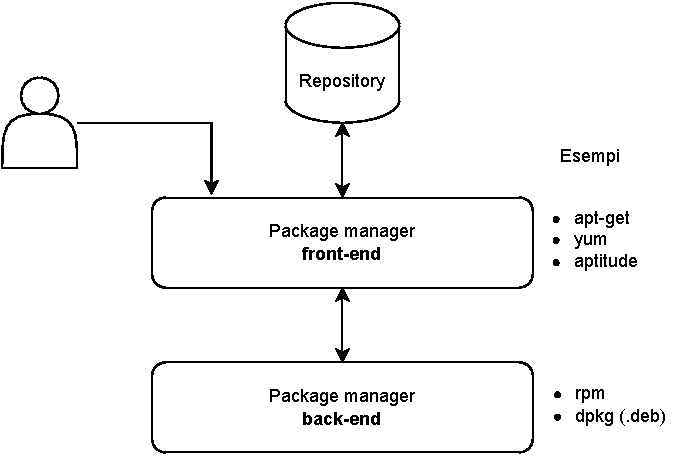
\includegraphics[width=.7\linewidth]{figures/package-managers.pdf}
	\caption{Struttura più diffusa dei sistemi di gestione di pacchetti}
	\label{fig:package-managers}
\end{figure}

Nei sistemi operativi Linux il gestore dei pacchetti è fondamentale per gestire gli applicativi ed i componenti del sistema, MacOs e Windows invece, offrono alternative di terze parti utilizzate maggiormente da utenti avanzati. Nei seguenti paragrafi saranno illustrati i principali repository utilizzabili per distribuire Alchemist.

\paragraph{Arch User Repository} Una distribuzione importante nel vasto panorama dei fork Linux è Arch. Arch è una distribuzione Linux con architettura x86-64 creata seguendo la filosofia \ac{kiss}. È infatti rinomata per essere leggera, veloce, estremamente scalabile ed adattabile alle proprie esigenze. Data la sua natura minimalista, l'installazione iniziale non incorpora alcun strumento di configurazione automatica, nessun ambiente desktop e nessun altro strumento necessario all'avvio del sistema. Il sistema di gestione dei pacchetti si chiama \textit{pacman} ed a differenza dei concorrenti, opera sia a basso che ad alto livello. Un pacchetto non è altro che un file shell script denominato \textit{PKGBUILD} contenente le istruzioni necessarie a scaricare i sorgenti e compilarli attraverso un comando: \textit{makepkg}. La linearità dei file PKGBUILD rende la creazione di pacchetti alla portata di qualsiasi utente difatti Arch supporta l'\textbf{\ac{aur}}, un tratto distintivo di questa distribuzione. Si tratta di un repository di pacchetti in cui qualsiasi utente, anche non sviluppatore, può contribuire.  

\paragraph{Windows e winget} Discorso differente vale per Windows, ove fino a poco tempo fa non era previsto alcun package manager ufficiale pre-installato. Gli utenti usualmente installano software attraverso pacchetti distribuiti in siti web ad-hoc, store non ufficiali o attraverso il Microsoft Store, gli sviluppatori invece, per sfruttare tutti i benefici della gestione a pacchetti utilizzano package-management system di terze parti. Solamente nel settembre 2020 è nato ``winget": package-management system open-source sviluppato da Microsoft, il quale supporta pacchetti di installazione EXE, MSIX e MSI. Il repository dei pacchetti è accessibile pubblicamente ed è possibile mediante richieste di contribuzione e previa approvazione, pubblicare pacchetti all'interno di esso.

\paragraph{Pacchetti containerizzati} Un'altra tipologia sono i pacchetti detti containerizzati, ovvero eseguiti all'interno di ambienti separati con un accesso limitato al sistema. Questa caratteristica fornisce due principali vantaggi: la possibilità per una applicazione di usare la propria versione desiderata di librerie di sistema senza creare conflitti e la trasparenza all'utente nell'accesso alle risorse di sistema, garantendo un livello aggiuntivo di sicurezza. È il caso dei pacchetti \textit{snap}, pacchetti auto-contenuti considerati universali perché compatibili con una notevole quantità di distribuzioni Linux. Quest'ultimi sono disponibili ed installabili all'interno dello ``SnapStore", l'unico repository compatibile ed ufficiale.

\paragraph{Analisi rispetto ai requisiti}
Nell'ottica di soddisfare il requisito multi-piat\-ta\-for\-ma del progetto è necessario analizzare le piattaforme di destinazione elencate. Data la natura closed-source di Windows e MacOs, i due sistemi operativi non richiedono particolari attenzioni dato che le tipologie di pacchetti generabili da jpackage sono sufficienti ed ufficialmente supportate. Linux al contrario è notevolmente frammentato, ogni distribuzione è libera di utilizzare il package management system preferito o di inventare una tipologia di pacchetto completamente nuova. Purtroppo non esistono statistiche ufficiali riguardo la diffusione delle distribuzioni, molte di esse si basano su stime o utilizzano dati non attendibili. Dall'altro lato analizzando i pacchetti generabili da jpackage possiamo trarre delle conclusioni.
\begin{itemize}
	\item RPM significa ``RedHat Package Manager", è un formato dei pacchetti progettato per RedHat e le distribuzioni derivate, risulta diffuso inoltre su Fedora, CentOs, OpenSUSE e tante altre distribuzioni. 
	\item DEB è l'abbreviazione di ``Debian packages", è una tipologia di pacchetto supportata da Debian e le distribuzioni derivate. Secondo distrowatch\footnote{https://distrowatch.com/} Debian Linux presenta più di 400 distribuzioni derivate e più di 120 di queste sono attive.
\end{itemize}
È evidente come le due tipologie coprono un ampio spettro nel panorama Linux. Esse inoltre sono supportate nativamente da PKGBUILD e rappresentano la totalità dei pacchetti generabili attraverso il software jpackage. Pertanto le due tipologie rappresenteranno la distribuzione per i sistemi Linux. Il supporto aggiuntivo ai pacchetti \textit{snap} fornisce un ulteriore livello di compatibilità essendo di fatto considerato una tipologia universale nel mondo Linux.

